\documentclass[11pt]{article}
\usepackage{geometry} 
\geometry{a4paper,top=3cm,bottom=3cm,left=2.5cm,right=2.5cm}   
\usepackage{multicol}
\usepackage[english, italian]{babel}
\usepackage{fancyhdr}
\usepackage{musicography}
\geometry{centering}
\usepackage{graphicx}


\pagestyle{fancy}                                 %serve ad inserire la linea sopra e il titolino
\rhead{\textsf{Lezione 2 "\textit{fondamenti dell'audio digitale 1}"}}
\renewcommand{\headrulewidth}{5pt} %grandezza della linea in alto
\renewcommand{\footrulewidth}{1pt}   % grandezza della linea in basso


\begin{document}
\begin{minipage}{0.55\linewidth}
\vspace{0.3cm}
{\large{\textbf{\textsf{Gabriele Petrillo}}}}\\\end{minipage}

\vspace{0.3cm}
\begin{minipage}{0.95\linewidth}
\begin{center}
{\huge{\textbf{\textsf{Fondamenti dell'audio digitale 1}}}} \\
\end{center}
\end{minipage}
\vspace*{0.2cm}


%=========ABSTRACT=======================
\begin{center}
\begin{minipage}[c]{14cm}
\begin{textit}

Ciò che segue è stato sviluppato a partire dalla dispensa di composizione del 25/11/2019 del prof. N.Bernardini presso il conservatorio S.Cecilia di Roma che possono essere consultati presso https://github.com/SMERM/TR-2019-2020/tree/master/A.A.2019-2020/COME-02/20191125. L'argomento trattato è il campionamento di un segnale audio e il problema dell'aliasing con dimostrazioni ed esempi in Octave.

\end{textit}
\end{minipage}
\end{center}
\vspace*{0.2cm}

%=========ARTICOLO========================

\begin{multicols*}{2}
\parskip=0pt

\textbf{\textsf {Campionamento}}\\

\noindent Un segnale analogico in uscita da un microfono è un segnale elettrico che descrive in maniera continua un onda acustica.  I segnali digitali sono dei segnali descritti da una serie di valori discreti che rappresentano, nel nostro caso, il valore che una pressione sonora ha in un determinato istante di tempo. Per processare il suono con il computer è necessario convertire il segnale analogico in digitale quindi in un flusso di valori numerici binari che può essere scritto nella memoria di un computer. Questo processo si chiama conversione analogico/digitale ed è eseguita da un convertitore chiamato \textbf{ADC}  (analog to digital converter).

Per convertire il segnale analogico in digitale è necessario misurare il segnale ad intervalli di tempo regolari, questo processo è detto \textbf{campionamento}.
L'intervallo di tempo fra un campione ed il successivo si chiama \textbf{periodo di campionamento} e si misura in secondi. L'inverso del periodo di campionamento, cioè il numero di volte che il segnale viene campionato in un secondo, è chiamato \textbf{frequenza di campionamento} (sample rate) ed è misurata in Hz (fig 1).

È chiaro che una buona rappresentazione del segnale è formata da tanti campioni e più campioni vengono presi in considerazione più accurata sarà la rappresentazione. Tuttavia, per capire qual è la frequenza di 
campionamento che permette un campionamento corretto del segnale, non potendone effettuare uno infinito, dobbiamo rifarci al teorema di Nyquist.

\begin{center}
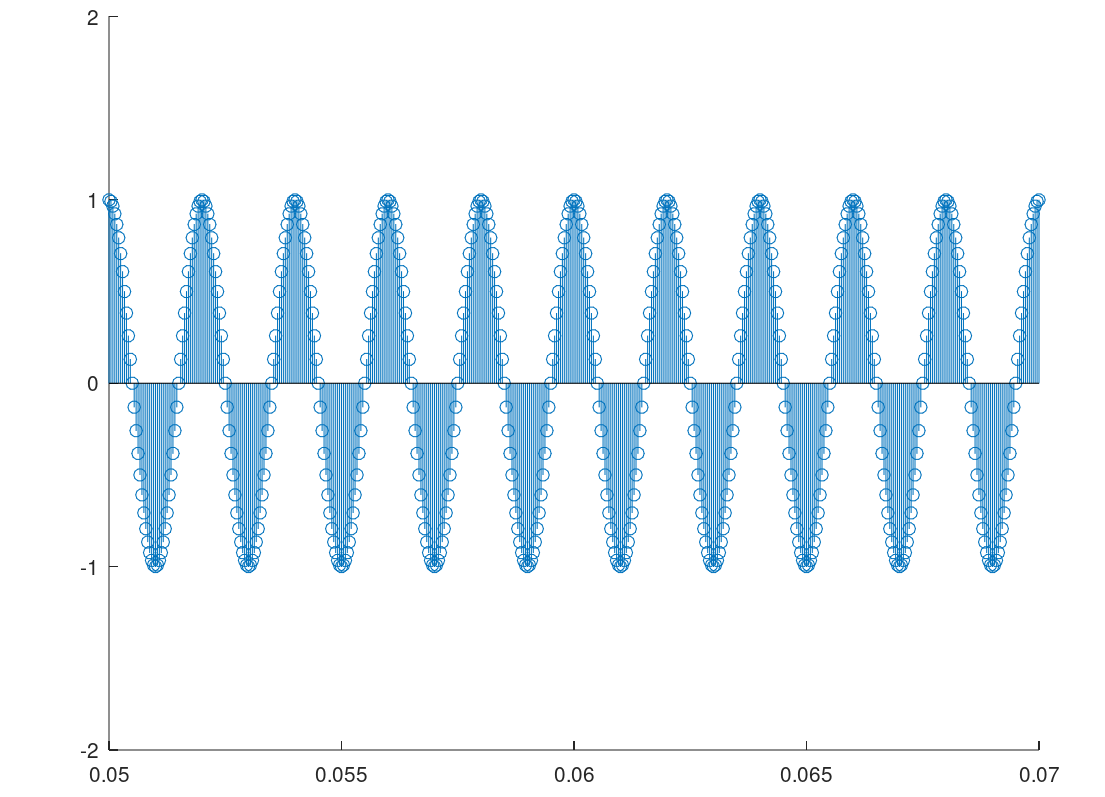
\includegraphics[scale=0.2]{images/plot02.png}

{\scriptsize \emph{fig.1 }}
\end{center}

\noindent Questo teorema afferma che, per non introdurre nessun errore, è necessario campionare ad una frequenza almeno doppia della frequenza massima contenuta nel segnale analogico. La relazione sarà quindi: 
\[
sr\ge 2* f_{max}
\]

\noindent Questa frequenza è chiamata \textbf{frequenza di Nyquist}.

Per essere sicuri che la frequenza più alta nel segnale analogico sia al di sotto della frequenza di Nyquist, bisogna applicare al segnale analogico un filtro passa basso con frequenza di taglio pari alla frequenza di Nyquist prima del convertitore ADC. Questo filtro viene chiamato \textbf{filtro anti-aliasing}.  \\

\textbf{\textsf {Ex.1 Cosinusoide in Octave}}\\

\noindent Proviamo a stampare in Octave il grafico di una cosinusoide a 200Hz con frequenza di campionamento pari a 48000 Hz in un intervallo di tempo pari a 0.1 sec.
Per fare questo dobbiamo:

\begin{itemize}
\item Scrivere un array di valori che rappresenta il campionamento nel dominio del tempo;
\item Inserire i valori della cosinusoide per tutti i punti
\end{itemize}

\noindent Definiamo prima tutte le variabili che ci serviranno:

\begin{center}
\begin{minipage}[c]{3cm}
\begin{sffamily}

fc = 48000;    \%sr\\
sinc = 1/fc;   \%T\\
dur = 0.1;      \%sec\\
freq = 200;    \%hz\\

\end{sffamily}
\end{minipage}
\end{center}

\noindent Adesso dobbiamo creare l’asse del tempo, che non è altro che un Array. In Octave gli Array vengono creati con le parentesi quadre, tuttavia inserire tutti i punti di campionamento sarebbe eccessivamente lungo, e per evitarlo possiamo utilizzare l’operatore (:) che ci permette di costruire un array di numeri che partono da un valore minimo ad un massimo con un determinato passo. Nel nostro caso dobbiamo creare dei valori che partono all’istante 0, arrivano all’istante \textit{dur - sinc} (questo perché i valori partono da 0, ma il conteggio del periodo di campionamento parte da 1) con un passo pari al periodo di campionamento, nel nostro caso la variabile \textit{sinc}.

\begin{center}
\begin{minipage}[c]{4cm}
\begin{sffamily}

t = [0:sinc:dur-sinc]; %asse del tempo

\end{sffamily}
\end{minipage}
\end{center}

\noindent Ora dobbiamo scrivere la funzione di una sinusoide:

\begin{center}
\begin{minipage}[c]{4cm}
\begin{sffamily}

y = cos(2*pi*freq*t);

\end{sffamily}
\end{minipage}
\end{center}

\noindent Moltiplicare un numero per un array significa moltiplicare questo numero per ogni valore dell’array, in questo caso noi otteniamo i valori della funzione coseno per ogni valore dell’array \textit{t}, ovvero ogni valore della nostra cosinusoide nel tempo ad una specifica frequenza di campionamento.
Per stampare il grafico, in Octave, è necessario usare il metodo \textit{plot( )} che per argomenti vuole i valori che andranno scritti rispettivamente sull’asse x e sull’asse y, in questo caso t e y:

\begin{center}
\begin{minipage}[c]{2cm}
\begin{sffamily}

plot (t,y)

\end{sffamily}
\end{minipage}
\end{center}

\noindent Per scalare il grafico possiamo usare il metodo \textit{axis( )}. Questo metodo prevede come argomento una lista con i valori estremi rispettivamente dell’asse x e y:

\begin{center}
\begin{minipage}[c]{4cm}
\begin{sffamily}

axis ([0.05 0.06 -2 2]) \\

\end{sffamily}
\end{minipage}
\end{center}

\begin{center}
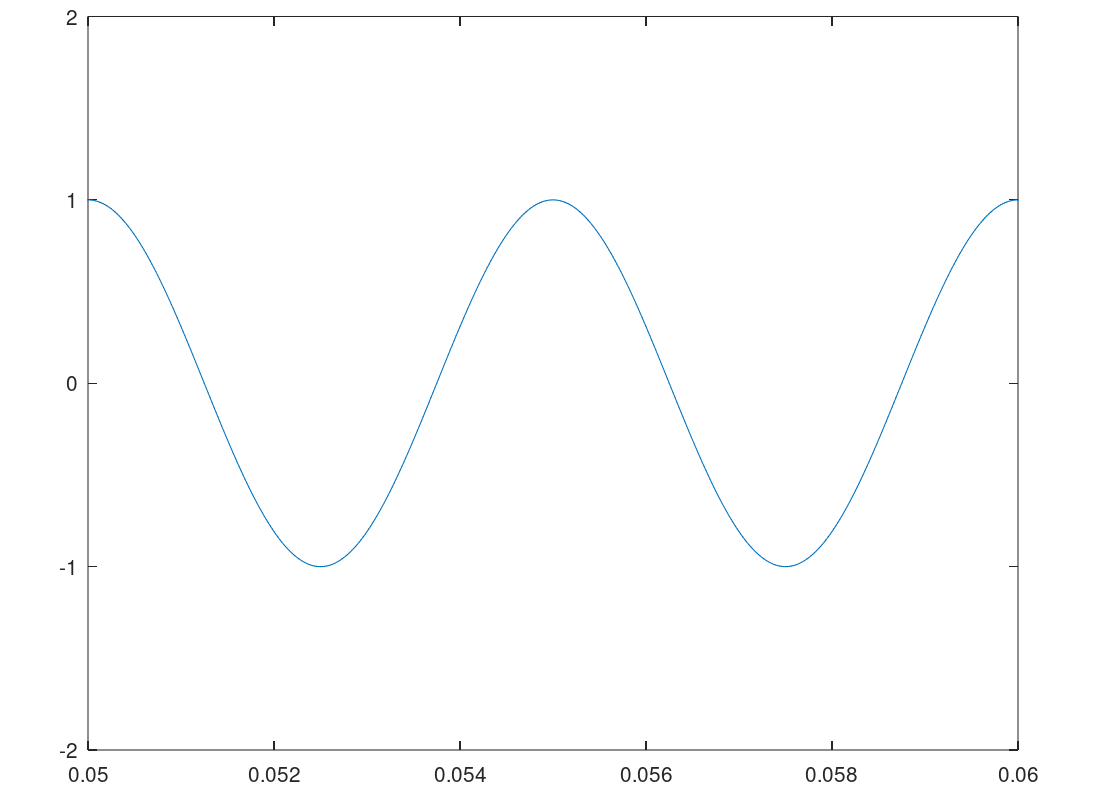
\includegraphics[scale=0.2]{images/plot01.png}

{\scriptsize \emph{fig.2 }}
\end{center}


\textbf{\textsf {Aliasing}}\\

\noindent Il problema di lavorare con sequenze di valori discreti è che la stessa serie di campioni possono essere condivisi da più segnali. Se infatti proviamo a campionare una sinusoide superiore alla frequenza di Nyquist quello che otteniamo è un effetto di \textit {foldover} (ripiegamento) alla frequenza di campionamento. Ad esempio se campioniamo una sinusoide di 402 Hz con una frequenza di campionamento di 400 Hz otteniamo una sinusoide di 1 Hz secondo la formula:

\[
f = f_c -  sr
\]

\noindent Dove \textit {f} è la frequenza generata, \textit f\ped{c} la frequenza da convertire e \textit {sr} la frequenza di campionamento. Queste frequenze causate dal sottocampionamento prendono il nome di \textit {alias}. 

Per evitare questo fenomeno è necessario usare il filtro anti-aliasing al segnale in ingresso al convertitore in modo da eliminare tutte le frequenze superiori alla frequenza di Nyquist ed evitare gli effetti di \textit {foldover}, infatti una volta che queste frequenze vengono create non c'è modo di risalire alla frequenza originale.\newpage

\textbf{\textsf {Ex.2 Foldover}} \\

\noindent Verifichiamo il foldover. Secondo la teoria campionando una cosinusoide a 401 Hz con una frequenza di campionamento di 400 Hz dovremmo ottenere una cosinusoide di 1 Hz dovuta dalla riflessione delle frequenze che superano la frequenza di Nyquist. Quindi impostiamo il programma esattamente come prima e verifichiamo il fenomeno:

\begin{center}
\begin{minipage}[c]{5cm}
\begin{sffamily}

fc = 400;    \%sr\\
sinc = 1/fc;   \%T\\
dur = 1;      \%sec\\
freq = 401;    \%hz\\
t = [0:sinc:dur-sinc]; \%asse x\\
y = cos (2*pi*freq*t); \%cos
stem (t,y)

\end{sffamily}
\end{minipage}
\end{center}

\noindent Per stampare questo grafico abbiamo usato il metodo \textit {stem ( )} che è molto simile a \textit {plot}, richiede gli stessi argomenti, ma stampa le proiezioni dei valori di y sull’asse x:

\begin{center}
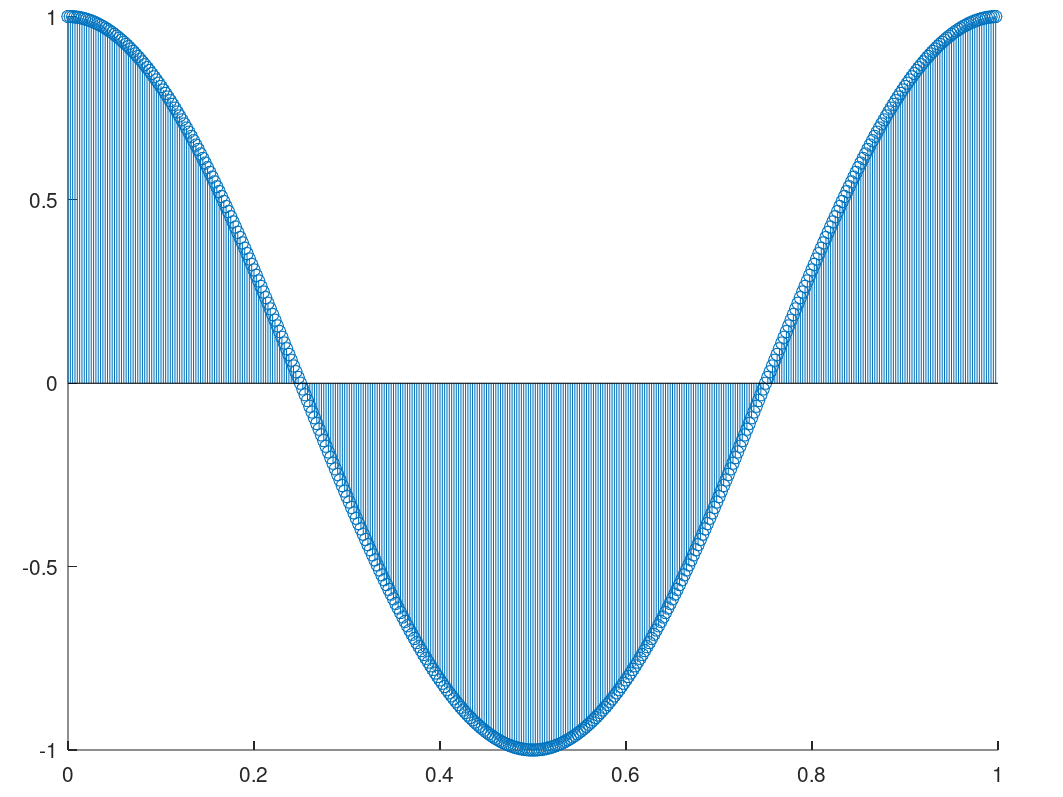
\includegraphics[scale=0.2]{images/plot03.png}

{\scriptsize \emph{fig.3 }}
\end{center}

\textbf{\textsf {Ex.3 Aliasing}}\\

\noindent Se sottocampioniamo una frequenza ne otteniamo un'altra che avrà in comune con l’originale i valori campionati secondo la regola $f = f_c + (k * sr)$ in cui \textit k sono tutti i multipli interi della frequenza di campionamento. Ad esempio una cosinusoide con frequenza 802 Hz campionata a 48000 e sottocampionata a 400 Hz, genera due frequenze diverse ma che hanno dei punti in comune. Impostiamo il programma come sopra specificando i valori di campionamento per entrambe le frequenze:

\begin{center}
\begin{minipage}[c]{6cm}
\begin{sffamily}

fc1 = 48000; \%sr1\\
fc2 = 400; \%sr2\\
sinc1 = 1/fc1; \%T1\\
sinc2 = 1/fc2; \%T2\\
dur = 1;  \%sec\\
freq = 802;  \%freq.\\
t1 = [0:sinc1:dur-sinc1]; \%asse x1\\
t2 = [0:sinc2:dur-sinc2]; \%asse x2\\
y1 = cos (2*pi*t1*freq); \%cos1\\
y2 = cos (2*pi*t2*freq); \%cos2\\
hold on\\
plot (t1,y1)\\
axis ([0.05 0.07])\\
stem (t2,y2) \\
hold off\\

\end{sffamily}
\end{minipage}
\end{center}

\noindent Per stampare entrambe le cosinusoidi sullo stesso grafico è necessario utilizzare la funzione \textit {hold on} prima dei vari metodi \textit {plot} o \textit {stem} ed infine \textit {hold off}. In questo modo possiamo stampare sullo stesso grafico il plot della prima cosinusoide e le proiezioni dei valori della seconda sinusoide del valore di 2 Hz $((802 - 400)-400$, viene infatti ripagata due volte).

\begin{center}
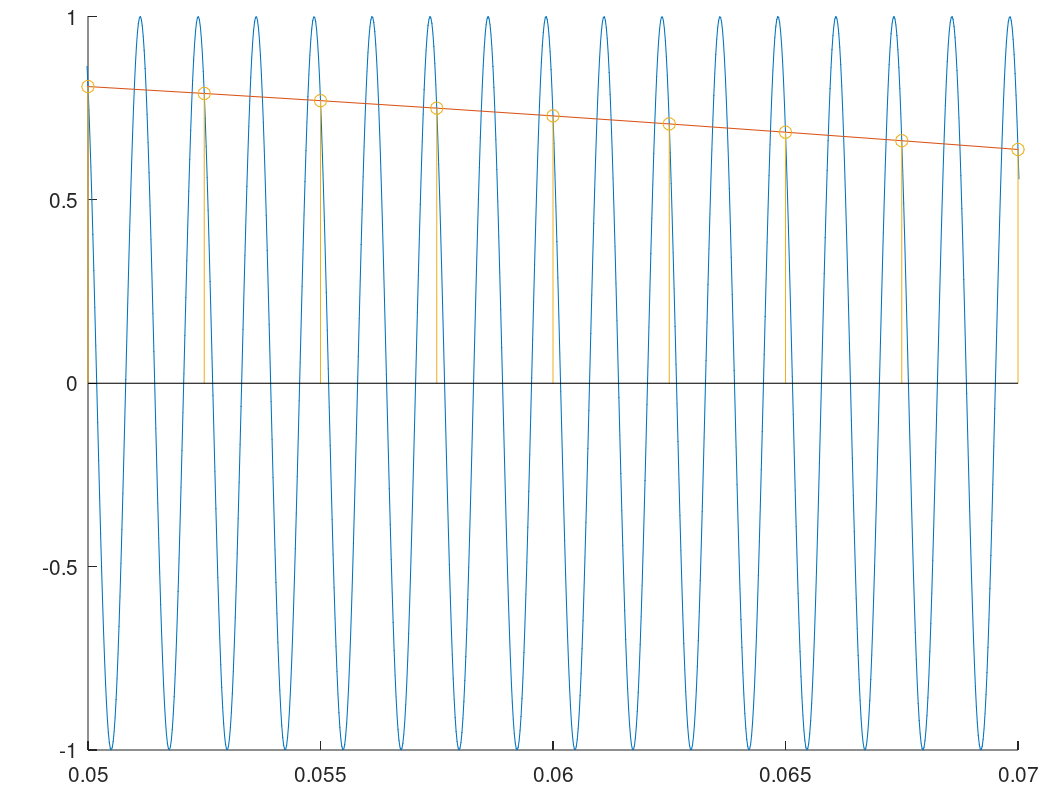
\includegraphics[scale=0.2]{images/plot04.png}

{\scriptsize \emph{fig.3 }}
\end{center}

\textbf{\textsf {Ex.4 freq. di campionamento}}\\

\noindent Per avere un campionamento corretto, dobbiamo campionare almeno a 44100 Hz. Proviamo quindi a campionare un file audio variando nel tempo la frequenza di campionamento in 1, 10, 100, 1000, 10000, 22050 e 44100 Hz per vedere cosa succede al file audio. Questo script è abbastanza complesso iniziamo analizzando la funzione \textit {audioread} e \textit {audiowrite} di Octave che permettono di leggere e scrivere audio in vari formati (wav, Flac e ogg vorbis). 

Per utilizzare questa funzione dobbiamo innanzitutto controllare che il file da leggere sia nel percorso di Octave, quindi scriviamo \textit {(ls .)} per vedere in quale percorso siamo, nel caso non sia quello giusto possiamo specificarlo con \textit {cd <folder>}. Per utilizzare la funzione \textit {audioread} dobbiamo specificare il nome degli array in cui la funzione \textit {audioread} ritornerà tutti i valori, rispettivamente il valore dei campioni (nel nostro caso \textit {snd}) e la frequenza di campionamento (nel nostro caso \textit {fc}), poi dobbiamo inserire come attributo di audioread il nome del file:

\vspace{0.3cm}

\begin{center}
\begin{minipage}[c]{6cm}
\begin{sffamily}

[snd fc] = audioread (“babay.wav”); \\

\end{sffamily}
\end{minipage}
\end{center}

\noindent A questo punto dobbiamo specificare un array di valori che corrisponde alle frequenze di campionamento che vogliamo utilizzare:

\vspace{0.3cm}

\begin{center}
\begin{minipage}[c]{6cm}
\begin{sffamily}

fcs = [1 10 100 1000 10000 22050 44100]; \\

\end{sffamily}
\end{minipage}
\end{center}

\noindent Adesso quello che a noi serve è conoscere la durata in secondi del brano e creare una matrice di output pari al prodotto del numero degli elementi dell’array \textit {snd} e il numero degli elementi dell’array \textit {fcs}, in quanto noi vogliamo leggere lo stesso file, quindi la stesso numero di campioni, un numero di volte pari alle frequenze di campionamento da sperimentare. Per calcolare la durata è sufficiente dividere il numero di campioni del file per la frequenza di campionamento, però per conoscere il numero dei campioni dobbiamo usare il metodo \textit {length( )} che ritorna il numero di elementi contenuto in un array (nel nostro caso \textit{snd}):

\vspace{0.3cm}

\begin{center}
\begin{minipage}[c]{4cm}
\begin{sffamily}

dur = length(snd)/fc; \\

\end{sffamily}
\end{minipage}
\end{center}

\noindent Per creare una matrice possiamo utilizzare il metodo \textit {zeros( )} che ritorna una matrice della lunghezza espressa negli argomenti contenente tutti 0, come argomenti vuole il numero degli elementi ed il numero di colonne, nel nostro caso 1, che poi andremo a sostituire con i valori dei campioni:

\vspace{0.3cm}

\begin{center}
\begin{minipage}[c]{7cm}
\begin{sffamily}

out = zeros(length(snd)*length(fcs),1);  \\

\end{sffamily}
\end{minipage}
\end{center}

\noindent Per scrivere i dati all’interno dell’array possiamo utilizzare un ciclo for. In Octave la sintassi del ciclo for è: for \textit {indice=valore iniziale dell’indice : valore massimo}. A capo va inserito il gruppo di istruzioni da eseguire e si conclude con la keyword \textit {end}. Quello che dobbiamo fare è compilare la matrice out sette volte, una volta per ogni frequenza di campionamento, quindi dobbiamo prima scegliere la prima frequenza di campionamento e scrivere tutti i campioni, poi scorrere alla seconda e compilare tutti gli altri campioni e così via. Per fare questo sono necessari due cicli for annidati, vediamo come:

\begin{center}
\begin{minipage}[c]{8cm}
\begin{sffamily}


For k = 1:length(fcs)\\
	curfc = fcs(k); \%sr corrente\\
	cursinc = round(fc/curfc); \%T corrente\\
	globalstart = length(snd)*(k-1);\\
	\%campione di inizio di ogni sezione relativa a fcs\\
	m = 0; \%campione di inizio\\
	for n = 1:cursinc:length(snd)\\
		tmpout = ones(cursinc,1)*snd(n);\\
		\%valore dei campioni a step\\
		startsnd = globstart+m*cursinc+1;\\
		\%inizio di ogni blocco di campioni\\
		out(startsnd:startsnd+length(tmpout)-1,1)=tmpout;\\
		m+=1;\\
	end\\
End\\

\end{sffamily}
\end{minipage}
\end{center}

\noindent Lo script si può leggere in questo modo: per indice \textit k che ha come valore iniziale 1 arrivare al valore massimo pari agli elementi di \textit {fcs} (le nostre frequenze di campionamento quindi 7). Questo primo ciclo for ci serve infatti per scorrere tutte le frequenze di campionamento. Ad ogni iterazione dobbiamo creare una variabile con il valore della frequenza di campionamento corrente andando a cercare nell’array \textit fcs il valore corrispondente all’iterazione. In Octave per sapere il valore di un elemento di un array in base alla posizione basta identificare il nome dell’array e inserire come attributo la posizione dell’elemento, che nel nostro caso è espresso dal numero dell’iterazione, quindi \textit k:

\vspace{0.3cm}

\begin{center}
\begin{minipage}[c]{3cm}
\begin{sffamily}

curfc = fcs(k);\\

\end{sffamily}
\end{minipage}
\end{center}

\noindent Visto che non conosciamo la frequenza dei campionamento del file, possiamo esprimere il periodo di campionamento in campioni dividendo \textit {fc} (frequenza di campionamento originale) per \textit {curfc} (frequenza di campionamento corrente), tuttavia, visto che si tratta di un numero di campioni, è importante che non escano numeri con la virgola - a tal fine possiamo quindi usare il metodo round che arrotonda un numero float al numero integer più vicino:

\vspace{0.3cm}

\begin{center}
\begin{minipage}[c]{5cm}
\begin{sffamily}

cursinc = round(fc/curfc);\\

\end{sffamily}
\end{minipage}
\end{center}

\noindent Ogni frequenza di campionamento conterrà tutti i campioni del file audio, quindi dobbiamo specificare da quale posizione dell’array out il programma dovrà iniziare a scrivere i campioni corrispondenti alle frequenze di campionamento, quindi il numero dei campioni per (\textit {k-1}) in quanto dobbiamo partire da 0:

\vspace{0.3cm}

\begin{center}
\begin{minipage}[c]{6cm}
\begin{sffamily}

globalstart = length(snd)*(k-1);\\

\end{sffamily}
\end{minipage}
\end{center}

\noindent La variabile \textit m ci servirà come moltiplicatore per calcolare il campione di inizio di ogni periodo di campionamento, quindi è inizializzata a 0:

\vspace{0.3cm}

\begin{center}
\begin{minipage}[c]{2cm}
\begin{sffamily}

m = 0;\\

\end{sffamily}
\end{minipage}
\end{center}

\noindent Adesso ci serve un secondo ciclo for che viene attivato ad ogni ciclo del primo che serve a scrivere il valore di tutti i campioni di ogni iterazione del primo ciclo. Per indice \textit {n = 1} arrivare al numero degli elementi di snd con un passo pari al periodo di campionamento corrente corrente. Ad ogni iterazione dobbiamo creare un array grande quanto un periodo di campionamento in cui tutti i valori siano pari al primo valore campionato. Per fare questo dobbiamo utilizzare il metodo \textit {ones (  )} che in modo simile a \textit {zeros} crea un array con un numero di elementi specificati nell’attributo con valore 1 e moltiplicati per il valore di \textit {snd} pari al valore di \textit n (che rappresenta il primo valore del campione ogni periodo di campionamento):

\vspace{0.3cm}

\begin{center}
\begin{minipage}[c]{5.5cm}
\begin{sffamily}

tmpout = ones(cursinc,1)*snd(n);\\

\end{sffamily}
\end{minipage}
\end{center}

\noindent Ora dobbiamo scrivere ogni array di campioni per ogni periodo di campionamento sul giusto blocco di campioni corrispondenti che sarà uguale a m (il moltiplicatore del periodo) * il periodo di campionamento + 1 perché negli array la posizione degli elementi viene contata da 1 più il valore di \textit {globalstart} che equivale al primo campione di ogni iterazione delle frequenze di campionamento (quindi del primo ciclo for):

\vspace{0.3cm}

\begin{center}
\begin{minipage}[c]{6.3cm}
\begin{sffamily}

startsnd =. globalstart+m*cursinc+1;\\

\end{sffamily}
\end{minipage}
\end{center}

\noindent A questo punto non dobbiamo fare altro che scrivere tutte le sottomatrici di out grandi quanto il numero di campioni che compongono un periodo di campionamento con i valori di tmpout. In Octave la sintassi per inserire i valori nelle sottomatrici è il nome della matrice con attributo la posizione di partenza: la posizione di arrivo, la colonna di appartenenza uguale ai valori da inserire. Nel nostro caso avremo quindi il primo campione del ciclo \textit {startsnd} : il campione finale pari alla somma del primo con la lunghezza degli elementi che compongono il periodo di campionamento \textit {tmpout - 1} uguale ai valori da inserire \textit {tmpout}:

\vspace{0.3cm}

\begin{center}
\begin{minipage}[c]{7cm}
\begin{sffamily}

out(startsnd:startsnd+length(tmpout)-1,1)\\=tmpout;

\end{sffamily}
\end{minipage}
\end{center}

\noindent A questo punto manca solo da aumentare di 1 il valore m:

\vspace{0.3cm}

\begin{center}
\begin{minipage}[c]{2cm}
\begin{sffamily}

m += 1\\

\end{sffamily}
\end{minipage}
\end{center}

\noindent Per scrivere il file audio dobbiamo usare la funzione \textit {audiowrite} che richiede come argomenti il nome del file, il valore dei campioni e la frequenza di campionamento:

\vspace{0.3cm}

\begin{center}
\begin{minipage}[c]{5cm}
\begin{sffamily}

audiowrite(“babay2.wav”,out,fc);\\

\end{sffamily}
\end{minipage}
\end{center}

\noindent Per creare un grafico di un file audio dobbiamo prima di tutto leggere con autoread il file audio:

\vspace{0.3cm}

\begin{center}
\begin{minipage}[c]{6cm}
\begin{sffamily}

[y, fs] = audioread(“babay2.wav”);\\

\end{sffamily}
\end{minipage}
\end{center}

\noindent Successivamente dobbiamo fare la stessa cosa fatta negli esempi precedenti ma utilizzando per l’asse delle \textit y il valore \textit y di audioread e per l’asse \textit x i valori dell’array \textit t in cui il tempo è il periodo di campionamento per il numero degli elementi di \textit y:

\vspace{0.3cm}

\begin{center}
\begin{minipage}[c]{6cm}
\begin{sffamily}

dt = 1/fs; \\
t = 0: dt: (length(y)*dt)-dt;\\
plot(t,y)\\

\end{sffamily}
\end{minipage}
\end{center}

\begin{center}
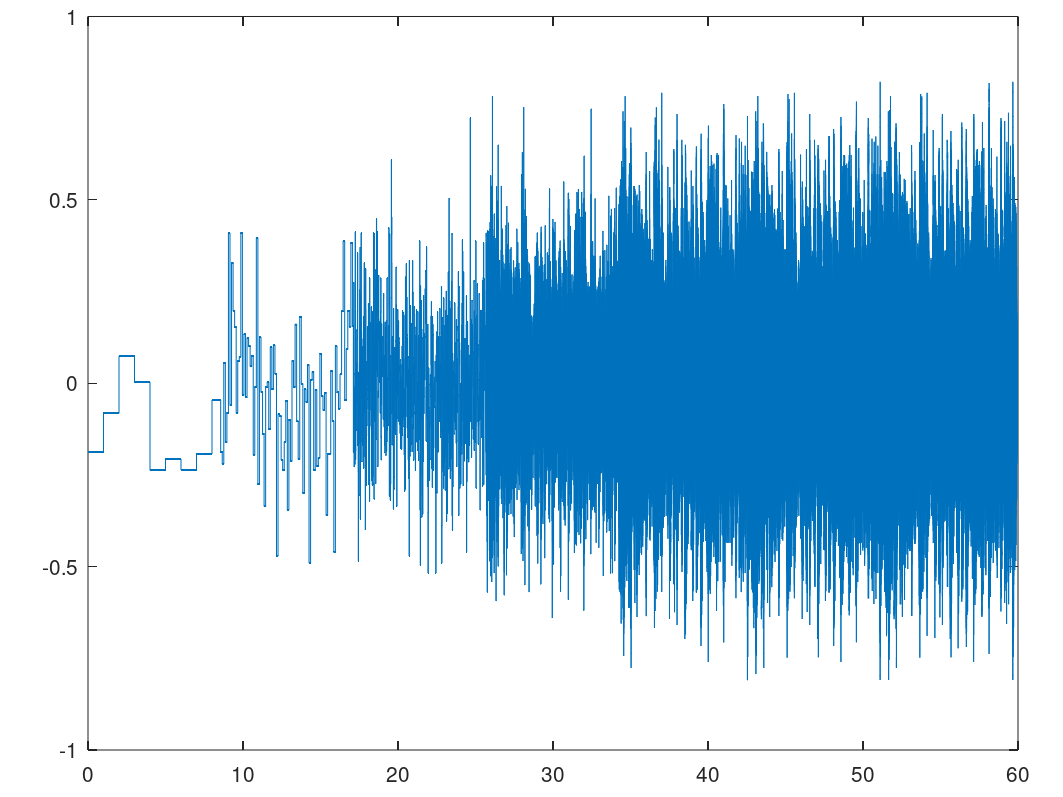
\includegraphics[scale=0.2]{images/plot05.png}

{\scriptsize \emph{fig.1 }}
\end{center}


\section*{\centering\small{BIBLIOGRAFIA}}
•\textsc{\textsf {Dodge, Charles and Jerse, Thomas A}}, \emph{Computer music: synthesis, composition and performance}, Macmillan Library Reference 1997\\
•\textsc{\textsf {Roads, Curtis and Strawn, John and others}}, \emph{The computer music tutorial}, MIT press, Editor 1996\\
•\textsc{\textsf {Bianchini, Riccardo and Cipriani, Alessandro}}, \emph{Il suono virtuale}, Contemponet 2001\\
•\textsc{\textsf {Cipriani, Alessandro and Giri Maurizio}}, \emph{Musica Elettronica e Sound Design}, Contemponet 2012\\
•\textsc{\textsf {Luise, Marco and Vitetta, Giorgio M.}}, \emph{Teoria dei Segnali}, McGraw-Hill 2009\\

\end{multicols*}

\end{document}